\documentclass[11pt,fleqn]{book} % Default font size and left-justified equations

\usepackage[top=3cm,bottom=3cm,left=3.2cm,right=3.2cm,headsep=10pt,a4paper]{geometry} % Page margins

\usepackage{xcolor,lipsum} % Required for specifying colors by name
\definecolor{ocre}{RGB}{0,56,102} 
\definecolor{lightgray}{RGB}{229,229,229} 
% Font Settings
\usepackage{avant} % Use the Avantgarde font for headings
%\usepackage{times} % Use the Times font for headings
\usepackage{mathptmx} % Use the Adobe Times Roman as the default text font together with math symbols from the Sym­bol, Chancery and Com­puter Modern fonts

\usepackage{microtype} % Slightly tweak font spacing for aesthetics
\usepackage[utf8]{inputenc}
\usepackage[T1]{fontenc} % Use 8-bit encoding that has 256 glyphs
\usepackage{hyperref}
\usepackage{empheq}
\usepackage{color}
\usepackage{caption}
\usepackage{afterpage}
\newcommand{\boxeq}[2]{\begin{empheq}[box=\colorbox{ocre!30}]{align}\label{#1}#2\end{empheq}}
\newcommand*{\xdash}[1][8em]{\rule[0.5ex]{#1}{0.55pt}}
\usepackage{makeidx}
\makeindex

% MATHS PACKAGE
\usepackage{amsmath,tikz}
\usetikzlibrary{matrix}
\newcommand*{\horzbar}{\rule[0.05ex]{2.5ex}{0.5pt}}
\usepackage{calc}

% VERBATIM PACKAGE
\usepackage{verbatim}
\usepackage{wrapfig}

%----------------------------------------------------------------------------------------
%	VARIOUS REQUIRED PACKAGES
%----------------------------------------------------------------------------------------

\usepackage{titlesec} % Allows customization of titles

\usepackage{graphicx} % Required for including pictures
\graphicspath{{Pictures/}} % Specifies the directory where pictures are stored

\usepackage{lipsum} % Inserts dummy text

\usepackage{tikz} % Required for drawing custom shapes

\usepackage[slovene]{babel} % English language/hyphenation

\usepackage{enumitem} % Customize lists
\setlist{nolistsep} % Reduce spacing between bullet points and numbered lists

\usepackage{booktabs} % Required for nicer horizontal rules in tables

\usepackage{eso-pic} % Required for specifying an image background in the title page

%\usepackage{draftwatermark}

%----------------------------------------------------------------------------------------
%	MAIN TABLE OF CONTENTS
%----------------------------------------------------------------------------------------

\usepackage{titletoc} % Required for manipulating the table of contents

\contentsmargin{0cm} % Removes the default margin
% Chapter text styling
\titlecontents{chapter}[1.25cm] % Indentation
{\addvspace{15pt}\large\sffamily\bfseries} % Spacing and font options for chapters
{\color{ocre!60}\contentslabel[\Large\thecontentslabel]{1.25cm}\color{ocre}} % Chapter number
{}  
{\color{ocre!60}\normalsize\sffamily\bfseries\;\titlerule*[.5pc]{.}\;\thecontentspage} % Page number
% Section text styling
\titlecontents{section}[1.25cm] % Indentation
{\addvspace{5pt}\sffamily\bfseries} % Spacing and font options for sections
{\contentslabel[\thecontentslabel]{1.25cm}} % Section number
{}
{\sffamily\hfill\color{black}\thecontentspage} % Page number
[]
% Subsection text styling
\titlecontents{subsection}[1.25cm] % Indentation
{\addvspace{1pt}\sffamily\small} % Spacing and font options for subsections
{\contentslabel[\thecontentslabel]{1.25cm}} % Subsection number
{}
{\sffamily\;\titlerule*[.5pc]{.}\;\thecontentspage} % Page number
[] 

%----------------------------------------------------------------------------------------
%	MINI TABLE OF CONTENTS IN CHAPTER HEADS
%----------------------------------------------------------------------------------------

% Section text styling
\titlecontents{lsection}[0em] % Indendating
{\footnotesize\sffamily} % Font settings
{}
{}
{}

% Subsection text styling
\titlecontents{lsubsection}[.5em] % Indentation
{\normalfont\footnotesize\sffamily} % Font settings
{}
{}
{}
 
%----------------------------------------------------------------------------------------
%	PAGE HEADERS
%----------------------------------------------------------------------------------------

\usepackage{fancyhdr} % Required for header and footer configuration

\pagestyle{fancy}
\renewcommand{\chaptermark}[1]{\markboth{\sffamily\normalsize\bfseries\chaptername\ \thechapter.\ #1}{}} % Chapter text font settings
\renewcommand{\sectionmark}[1]{\markright{\sffamily\normalsize\thesection\hspace{5pt}#1}{}} % Section text font settings
\fancyhf{} \fancyhead[LE,RO]{\sffamily\normalsize\thepage} % Font setting for the page number in the header
\fancyhead[LO]{\rightmark} % Print the nearest section name on the left side of odd pages
\fancyhead[RE]{\leftmark} % Print the current chapter name on the right side of even pages
\renewcommand{\headrulewidth}{0.5pt} % Width of the rule under the header
\addtolength{\headheight}{2.5pt} % Increase the spacing around the header slightly
\renewcommand{\footrulewidth}{0pt} % Removes the rule in the footer
\fancypagestyle{plain}{\fancyhead{}\renewcommand{\headrulewidth}{0pt}} % Style for when a plain pagestyle is specified

% Removes the header from odd empty pages at the end of chapters
\makeatletter
\renewcommand{\cleardoublepage}{
\clearpage\ifodd\c@page\else
\hbox{}
\vspace*{\fill}
\thispagestyle{empty}
\newpage
\fi}

%----------------------------------------------------------------------------------------
%	THEOREM STYLES
%----------------------------------------------------------------------------------------

\usepackage{amsmath,amsfonts,amssymb,amsthm} % For math equations, theorems, symbols, etc

\newcommand{\intoo}[2]{\mathopen{]}#1\,;#2\mathclose{[}}
\newcommand{\ud}{\mathop{\mathrm{{}d}}\mathopen{}}
\newcommand{\intff}[2]{\mathopen{[}#1\,;#2\mathclose{]}}
\newtheorem{notation}{Notation}[chapter]

%%%%%%%%%%%%%%%%%%%%%%%%%%%%%%%%%%%%%%%%%%%%%%%%%%%%%%%%%%%%%%%%%%%%%%%%%%%
%%%%%%%%%%%%%%%%%%%% dedicated to boxed/framed environements %%%%%%%%%%%%%%
%%%%%%%%%%%%%%%%%%%%%%%%%%%%%%%%%%%%%%%%%%%%%%%%%%%%%%%%%%%%%%%%%%%%%%%%%%%
\newtheoremstyle{ocrenumbox}% % Theorem style name
{0pt}% Space above
{0pt}% Space below
{\normalfont}% % Body font
{}% Indent amount
{\small\bf\sffamily\color{ocre}}% % Theorem head font
{\;}% Punctuation after theorem head
{0.25em}% Space after theorem head
{\small\sffamily\color{ocre}\thmname{#1}\nobreakspace\thmnumber{\@ifnotempty{#1}{}\@upn{#2}}% Theorem text (e.g. Theorem 2.1)
\thmnote{\nobreakspace\the\thm@notefont\sffamily\bfseries\color{black}---\nobreakspace#3.}} % Optional theorem note
\renewcommand{\qedsymbol}{$\blacksquare$}% Optional qed square

\newtheoremstyle{blacknumex}% Theorem style name
{5pt}% Space above
{5pt}% Space below
{\normalfont}% Body font
{} % Indent amount
{\small\bf\sffamily}% Theorem head font
{\;}% Punctuation after theorem head
{0.25em}% Space after theorem head
{\small\sffamily{\tiny\ensuremath{\blacksquare}}\nobreakspace\thmname{#1}\nobreakspace\thmnumber{\@ifnotempty{#1}{}\@upn{#2}}% Theorem text (e.g. Theorem 2.1)
\thmnote{\nobreakspace\the\thm@notefont\sffamily\bfseries---\nobreakspace#3.}}% Optional theorem note

\newtheoremstyle{blacknumbox} % Theorem style name
{0pt}% Space above
{0pt}% Space below
{\normalfont}% Body font
{}% Indent amount
{\small\bf\sffamily}% Theorem head font
{\;}% Punctuation after theorem head
{0.25em}% Space after theorem head
{\small\sffamily\thmname{#1}\nobreakspace\thmnumber{\@ifnotempty{#1}{}\@upn{#2}}% Theorem text (e.g. Theorem 2.1)
\thmnote{\nobreakspace\the\thm@notefont\sffamily\bfseries---\nobreakspace#3.}}% Optional theorem note

%%%%%%%%%%%%%%%%%%%%%%%%%%%%%%%%%%%%%%%%%%%%%%%%%%%%%%%%%%%%%%%%%%%%%%%%%%%
%%%%%%%%%%%%% dedicated to non-boxed/non-framed environements %%%%%%%%%%%%%
%%%%%%%%%%%%%%%%%%%%%%%%%%%%%%%%%%%%%%%%%%%%%%%%%%%%%%%%%%%%%%%%%%%%%%%%%%%
\newtheoremstyle{ocrenum}% % Theorem style name
{5pt}% Space above
{5pt}% Space below
{\normalfont}% % Body font
{}% Indent amount
{\small\bf\sffamily\color{ocre}}% % Theorem head font
{\;}% Punctuation after theorem head
{0.25em}% Space after theorem head
{\small\sffamily\color{ocre}\thmname{#1}\nobreakspace\thmnumber{\@ifnotempty{#1}{}\@upn{#2}}% Theorem text (e.g. Theorem 2.1)
\thmnote{\nobreakspace\the\thm@notefont\sffamily\bfseries\color{black}---\nobreakspace#3.}} % Optional theorem note
\renewcommand{\qedsymbol}{$\blacksquare$}% Optional qed square
\makeatother

% Defines the theorem text style for each type of theorem to one of the three styles above
\newcounter{dummy} 
\numberwithin{dummy}{section}
\theoremstyle{ocrenumbox}
\newtheorem{theoremeT}[dummy]{Theorem}
\newtheorem{problem}{Problem}[chapter]
\newtheorem{exerciseT}{Exercise}[chapter]
\theoremstyle{blacknumex}
\newtheorem{exampleT}{Example}[chapter]
\theoremstyle{blacknumbox}
\newtheorem{vocabulary}{Vocabulary}[chapter]
\newtheorem{definitionT}{Naloga}[section]
\newtheorem{corollaryT}[dummy]{Corollary}
\theoremstyle{ocrenum}
\newtheorem{proposition}[dummy]{Računski zgled}

%----------------------------------------------------------------------------------------
%	DEFINITION OF COLORED BOXES
%----------------------------------------------------------------------------------------

\RequirePackage[framemethod=default]{mdframed} % Required for creating the theorem, definition, exercise and corollary boxes

% Theorem box
\newmdenv[skipabove=7pt,
skipbelow=7pt,
backgroundcolor=black!5,
linecolor=ocre,
innerleftmargin=5pt,
innerrightmargin=5pt,
innertopmargin=5pt,
leftmargin=0cm,
rightmargin=0cm,
innerbottommargin=5pt]{tBox}

% Exercise box	  
\newmdenv[skipabove=7pt,
skipbelow=7pt,
rightline=false,
leftline=true,
topline=false,
bottomline=false,
backgroundcolor=ocre!10,
linecolor=ocre,
innerleftmargin=5pt,
innerrightmargin=5pt,
innertopmargin=5pt,
innerbottommargin=15pt,
leftmargin=0cm,
rightmargin=0cm,
linewidth=4pt]{eBox}	

% Definition box
\newmdenv[
skipabove=7pt,
skipbelow=7pt,
rightline=false,
leftline=false,
topline=true,
bottomline=true,
linecolor=ocre,
innerleftmargin=0pt,
innerrightmargin=0pt,
innertopmargin=15pt,
leftmargin=0cm,
rightmargin=0cm,
linewidth=1pt,
innerbottommargin=7pt]{dBox}	

% Corollary box
\newmdenv[skipabove=7pt,
skipbelow=7pt,
rightline=false,
leftline=true,
topline=true,
bottomline=true,
linecolor=red,
backgroundcolor=black!5,
innerleftmargin=5pt,
innerrightmargin=5pt,
innertopmargin=5pt,
leftmargin=0cm,
rightmargin=0cm,
linewidth=4pt,
innerbottommargin=5pt]{cBox}

% Creates an environment for each type of theorem and assigns it a theorem text style from the "Theorem Styles" section above and a colored box from above
\newenvironment{theorem}{\begin{tBox}\begin{theoremeT}}{\end{theoremeT}\end{tBox}}
\newenvironment{exercise}{\begin{eBox}\begin{exerciseT}}{\hfill{\color{ocre}\tiny\ensuremath{\blacksquare}}\end{exerciseT}\end{eBox}}				  
\newenvironment{definition}{\begin{dBox}\begin{definitionT}}{\end{definitionT}\end{dBox}}	
\newenvironment{example}{\begin{exampleT}}{\hfill{\tiny\ensuremath{\blacksquare}}\end{exampleT}}		
\newenvironment{corollary}{\begin{cBox}\begin{corollaryT}}{\end{corollaryT}\end{cBox}}	

%----------------------------------------------------------------------------------------
%	REMARK ENVIRONMENT
%----------------------------------------------------------------------------------------

\newenvironment{remark}{\par\vspace{10pt}\small % Vertical white space above the remark and smaller font size
\begin{list}{}{
\leftmargin=25pt % Indentation on the left
\rightmargin=0pt}\item\ignorespaces % Indentation on the right
\makebox[-2.5pt]{\begin{tikzpicture}[overlay]
\node[draw=ocre!60,line width=1pt,circle,fill=ocre!25,font=\sffamily\bfseries,inner sep=2pt,outer sep=0pt] at (-15pt,0pt){\textcolor{ocre}{$\bigstar$}};\end{tikzpicture}} % Orange R in a circle
\advance\baselineskip -1pt}{\end{list}\vskip5pt} % Tighter line spacing and white space after remark

%----------------------------------------------------------------------------------------
%	SECTION NUMBERING IN THE MARGIN
%----------------------------------------------------------------------------------------

\makeatletter
\renewcommand{\@seccntformat}[1]{\llap{\textcolor{ocre}{\csname the#1\endcsname}\hspace{1em}}}                    
\renewcommand{\section}{\@startsection{section}{1}{\z@}
{-4ex \@plus -1ex \@minus -.4ex}
{1ex \@plus.2ex }
{\normalfont\large\sffamily\bfseries}}
\renewcommand{\subsection}{\@startsection {subsection}{2}{\z@}
{-3ex \@plus -0.1ex \@minus -.4ex}
{0.5ex \@plus.2ex }
{\normalfont\sffamily\bfseries}}
\renewcommand{\subsubsection}{\@startsection {subsubsection}{3}{\z@}
{-2ex \@plus -0.1ex \@minus -.2ex}
{.2ex \@plus.2ex }
{\normalfont\small\sffamily\bfseries}}                        
\renewcommand\paragraph{\@startsection{paragraph}{4}{\z@}
{-2ex \@plus-.2ex \@minus .2ex}
{.1ex}
{\normalfont\small\sffamily\bfseries}}

%----------------------------------------------------------------------------------------
%	HYPERLINKS IN THE DOCUMENTS
%----------------------------------------------------------------------------------------

% For an unclear reason, the package should be loaded now and not later
\usepackage{hyperref}
\hypersetup{hidelinks,backref=true,pagebackref=true,hyperindex=true,colorlinks=true,breaklinks=true,urlcolor= ocre,linkcolor=ocre,bookmarks=true,bookmarksopen=false,pdftitle={Title},pdfauthor={Author}}

%----------------------------------------------------------------------------------------
%	CHAPTER HEADINGS
%----------------------------------------------------------------------------------------

% The set-up below should be (sadly) manually adapted to the overall margin page septup controlled by the geometry package loaded in the main.tex document. It is possible to implement below the dimensions used in the goemetry package (top,bottom,left,right)... TO BE DONE

\newcommand{\thechapterimage}{}
\newcommand{\chapterimage}[1]{\renewcommand{\thechapterimage}{#1}}

% Numbered chapters with mini tableofcontents
\def\thechapter{\arabic{chapter}}
\def\@makechapterhead#1{
\thispagestyle{empty}
{\centering \normalfont\sffamily
\ifnum \c@secnumdepth >\m@ne
\if@mainmatter
\startcontents
\begin{tikzpicture}[remember picture,overlay]
\node at (current page.north west)
{\begin{tikzpicture}[remember picture,overlay]
\node[anchor=north west,inner sep=0pt] at (0,0) {\includegraphics[width=\paperwidth]{\thechapterimage}};
%%%%%%%%%%%%%%%%%%%%%%%%%%%%%%%%%%%%%%%%%%%%%%%%%%%%%%%%%%%%%%%%%%%%%%%%%%%%%%%%%%%%%
% Commenting the 3 lines below removes the small contents box in the chapter heading
%\fill[color=ocre!10!white,opacity=.6] (1cm,0) rectangle (8cm,-7cm);
%\node[anchor=north west] at (1.1cm,.35cm) {\parbox[t][8cm][t]{6.5cm}{\huge\bfseries\flushleft \printcontents{l}{1}{\setcounter{tocdepth}{2}}}};
\draw[anchor=west] (3cm,-4cm) node [rounded corners=20pt,fill=ocre!10!white,text opacity=1,draw=ocre,draw opacity=1,line width=1.5pt,fill opacity=.6,inner sep=12pt]{\huge\sffamily\bfseries\textcolor{black}{\thechapter. #1\strut\makebox[22cm]{}}};
%%%%%%%%%%%%%%%%%%%%%%%%%%%%%%%%%%%%%%%%%%%%%%%%%%%%%%%%%%%%%%%%%%%%%%%%%%%%%%%%%%%%%
\end{tikzpicture}};
\end{tikzpicture}}
\par\vspace*{100\p@}
\fi
\fi}

% Unnumbered chapters without mini tableofcontents (could be added though) 
\def\@makeschapterhead#1{
\thispagestyle{empty}
{\centering \normalfont\sffamily
\ifnum \c@secnumdepth >\m@ne
\if@mainmatter
\begin{tikzpicture}[remember picture,overlay]
\node at (current page.north west)
{\begin{tikzpicture}[remember picture,overlay]
\node[anchor=north west,inner sep=0pt] at (0,0) {\includegraphics[width=\paperwidth]{\thechapterimage}};
\draw[anchor=west] (3cm,-4cm) node [rounded corners=20pt,fill=ocre!10!white,fill opacity=.6,inner sep=12pt,text opacity=1,draw=ocre,draw opacity=1,line width=1.5pt]{\huge\sffamily\bfseries\textcolor{black}{#1\strut\makebox[22cm]{}}};
\end{tikzpicture}};
\end{tikzpicture}}
\par\vspace*{80\p@}
\fi

\fi
}
\makeatother
 % Insert the commands.tex file which contains the majority of the structure behind the template

\newcommand{\beq}{\begin{equation}}
\newcommand{\eeq}{\end{equation}}   
\renewcommand{\arraystretch}{1.5}

\begin{document}

\let\cleardoublepage\clearpage

%--------------------------------------------------------------------------

%	TITLE PAGE
%--------------------------------------------------------------------------


\begingroup
\thispagestyle{empty}
%\AddToShipoutPicture*{\put(0,0){\includegraphics[scale=1.25]{v}}} % Image background
\centering
\vspace*{5cm}
\par\normalfont\fontsize{35}{35}\sffamily\selectfont
\textbf{FOTONIKA}\\
{\LARGE }\par % Book title
\vspace*{1cm}
{\LARGE Učno gradivo za študente \\ Fakultete za fiziko
\\ 
Univerze v Ljubljani\\}\par % Author name
\vspace*{1cm}
%{\LARGE \textcolor{red}{Delovna verzija}\\}\par
\vspace*{8cm}
{\Large Martin ČOPIČ \\Mojca VILFAN \\Andrej PETELIN \\}\par % Author name
\endgroup

%--------------------------------------------------------------------
%	COPYRIGHT PAGE
%-------------------------------------------------------------------

\newpage
~\vfill
\thispagestyle{empty}

%\noindent Copyright \copyright\ 2014 Andrea Hidalgo\\ % Copyright notice

\noindent Recenzenti: {***}\\ % Recenzent

\noindent Lektor: {***}\\ % Lektor

\noindent Risbe in diagrami: Andrej Petelin\\ % Risbe in diagrami

\noindent Naslovne fotografije poglavij: Mojca Vilfan\\ % Fotografije

\noindent \textit{\textcopyright 
Kopiranje in razmnoževanje besedila ali njegovih delov ter slik je 
dovoljeno samo z odobritvijo avtorjev knjige.} \\% Printing/edition date

\noindent \textsc{Ljubljana, *** 2016}\\

%-------------------------------------------------------------------
%	TABLE OF CONTENTS
%--------------------------------------------------------------------

\chapterimage{Slika.jpg} % heading image

\pagestyle{empty} % No headers

\renewcommand\contentsname{Kazalo}
\renewcommand{\bibname}{Bibliographie}
\tableofcontents% Print the table of contents itself

%\cleardoublepage % Forces the first chapter to start on an odd page so it's on 

\pagestyle{fancy} % Print headers again


%---------
%	PREDGOVOR
%-------------------------------------------------------------------------------

\chapterimage{Predgovor.jpg} % Chapter heading image

\chapter{Predgovor}

Fotonika ... 

Skozi celotno obravnavno svetlobe se bomo posluževali 
takih in drugačnih približkov. Tako bomo na primer pri obravnavi elektro-optičnih
pojavov pogosto uporabili približek ravnega vala. Za pojave, kjer vektorska narava 
elektromagnetnega valovanja ni ključnega pomena, bomo uporabili skalarno valovno teorijo. 
Kjer ne bo posebej omenjeno, bomo najpogosteje obravnavali homogeno izotropno snov, ki 
se linearno odziva na zunanje motnje. Sledila pa bodo cela poglavja, posvečena nelinearnim 
optičnim pojavom v snovi. \\

Svetlobo bomo torej opisali z elektromagnetnim valovanjem,
pri tem pa se moramo zavedati, da svetlobo lahko opišemo tudi s tokom
delcev - fotonov. Za pojave, kjer je kvantna narava svetlobe pomembna,
kot je recimo v fiziki laserjev, se moramo zateči h kvantni optiki.
Nekaj osnov kvantne optike bomo vpeljali kasneje, začnimo pa s
klasično obravnavo svetlobe - valovno enačbo za elektromagnetno polje.
\vspace{1em}

\noindent Avtorji

%-------------------------------------------------------------------------------

%	LITERATURA
%-------------------------------------------------------------------------------


\chapterimage{Lit.jpg} % Chapter heading image

\chapter{Priporočena dodatna literatura}

\begin{itemize}
\setlength\itemsep{0.5em}
 \item Saleh, Yariv, Silfvast, Davies. 
\end{itemize}

%-------------------------------------------------------------------------------
%	CHAPTER 1
%-------------------------------------------------------------------------------

\chapterimage{Slika.jpg} % Chapter heading image

\chapter{Elektromagnetno valovanje}

Za začetek osvežimo osnove teorije elektromagnetnega polja in elektromagnetnega valovanja. 
Obnovili bomo zapis Maxwellovih enačb, zapisali osnovne pojave valovanja (lom, odboj in uklon),
ter si ogledali razširanje svetlobe v anizotropnih snoveh. 

\section{Maxwellove enačbe}

Elektromagnetno polje v praznem prostoru opišemo z dvema vektorskima
poljema, električnim in magnetnim, ki sta v splošnem funkciji prostora
in časa. Vsaki točki v prostoru lahko priredimo \index{Električno polje!jakost}jakost
električnega polja $\mathbf{E}(\mathbf{r},t)$ in \index{Magnetno polje!jakost}jakost
magnetnega polja $\mathbf{H}(\mathbf{r},t)$. Za opis elektromagnetnega
polja v snovi vpeljemo dva dodatna vektorja polja. To sta \index{Električno polje!gostota}gostota
električnega polja $\mathbf{D}(\mathbf{r},t)$ in gostota magnetnega
polja\index{Magnetno polje!gostota} $\mathbf{B}(\mathbf{r},t)$.
Vsa ta polja povezujejo \index{Maxwellove enačbe}Maxwellove enačbe\footnote{
Škotski fizik James Clerk Maxwell, 1831-1879.}

\boxeq{eq:Maxwell1}{
\nabla\times\mathbf{H} & =\frac{\partial\mathbf{D}}{\partial t}+\mathbf{j_e}\\
\nabla\times\mathbf{E} & =-\frac{\partial\mathbf{B}}{\partial t}\label{eq:Maxwell2}\\
\nabla\cdot\mathbf{D} & =\mbox{\ensuremath{\rho}}_{e}\label{eq:Maxwell3}\\
\nabla\cdot\mathbf{B} & =0.\label{eq:Maxwell4}
}\\
V zapisu enačb smo upoštevali tudi izvore polj, to je gostoto
električnega toka $\mathbf{j}_e(\mathbf{r},t)$ in gostoto naboja $\rho_{e}(\mathbf{r},t)$. \\

\noindent
Poleg Maxwellovih enačb veljata za vektorski polji zvezi
\begin{align}
\mathbf{D} & =\epsilon_{0}\mathbf{E}+\mathbf{P}\\
\mathbf{B} & =\mu_{0}\mathbf{H}+\mu_{0}\mathbf{M},
\end{align}
kjer $\mathbf{P}$ označuje \index{Električna polarizacija}električno
polarizacijo, to je gostoto električnih dipolov, $\mathbf{M}$
pa \index{Magnetizacija}magnetizacijo, to je gostoto magnetnega momenta.
Polarizacija in magnetizacija sta odvisni od zunanjih polj $\mathbf{E}$
ter $\mathbf{H}$. V splošnem sta njuni odvisnosti zelo zapleteni,
v izotropnih in linearnih snoveh pa se zvezi poenostavita v 
\beq
\mathbf{P}=\epsilon_{0}\chi_e\mathbf{E} = \epsilon_{0}(\epsilon-1)\mathbf{E} \qquad \textrm{in} 
\qquad
\mathbf{M}=\chi_m \mathbf{H} = (\mu-1)\mathbf{H}.
\eeq
Vpeljali smo električno ($\chi_e$) in magnetno ($\chi_m$) susceptibilnost ter
\index{Dielektričnost}dielektričnost $\epsilon$ in
\index{Magnetna permeabilnost}magnetno permeabilnost $\mu$. Ko združimo gornje
enačbe, lahko zapišemo dve konstitutivni
relaciji
\begin{align}
\mathbf{D} & =\epsilon_{0}\epsilon\mathbf{E}\\
\mathbf{B} & =\mu_{0}\mu\mathbf{H}.
\end{align}
V linearnih anizotropnih snoveh moramo namesto skalarnih vrednosti $\varepsilon$
in $\mu$ zapisati tenzorje. 


\subsection*{Robni pogoji}
Navedene Maxwellove enačbe zadoščajo za opis elektromagnetnega polja
v neomejeni snovi, kjer so vse komponente polj zvezne funkcije. Za
obravnavo v omejeni snovi moramo vedeti tudi, kaj se z elektromagnetnim
poljem zgodi na meji dveh sredstev\index{Robni pogoji}. Pri prehodu
iz enega dielektrika v drugega se ohranjata normalni komponenti gostote
električnega in magnetnega polja ter tangentni komponenti jakosti
električnega in magnetnega polja (slika \ref{fig:Robni-pogoji}) 
\boxeq{eq:robni-pogoji}{
D_{1n} &=  D_{2n}\\
B_{1n} &=  B_{2n}\\
E_{1t} &=  E_{2t}\\
H_{1t} &=  H_{2t}.
}
Pri tem smo privzeli, da na meji med dielektrikoma ni površinskih
tokov ali nabojev, sicer bi morali robna pogoja za $D_n$ in $H_t$
ustrezno popraviti. Na meji dielektrika z idealnim prevodnikom (kovino,
zrcalom) so robni pogoji drugačni. Za magnetno polje jih ne moremo
preprosto zapisati, za električno polje pa velja, da mora biti tangentna
komponenta jakosti električnega polja enaka nič. Posledica tega robnega
pogoja je, da se pri pravokotnem vpadu valovanja na zrcalo faza valovanja
spremeni za $\pi$. 

\begin{figure}[h]
\centering
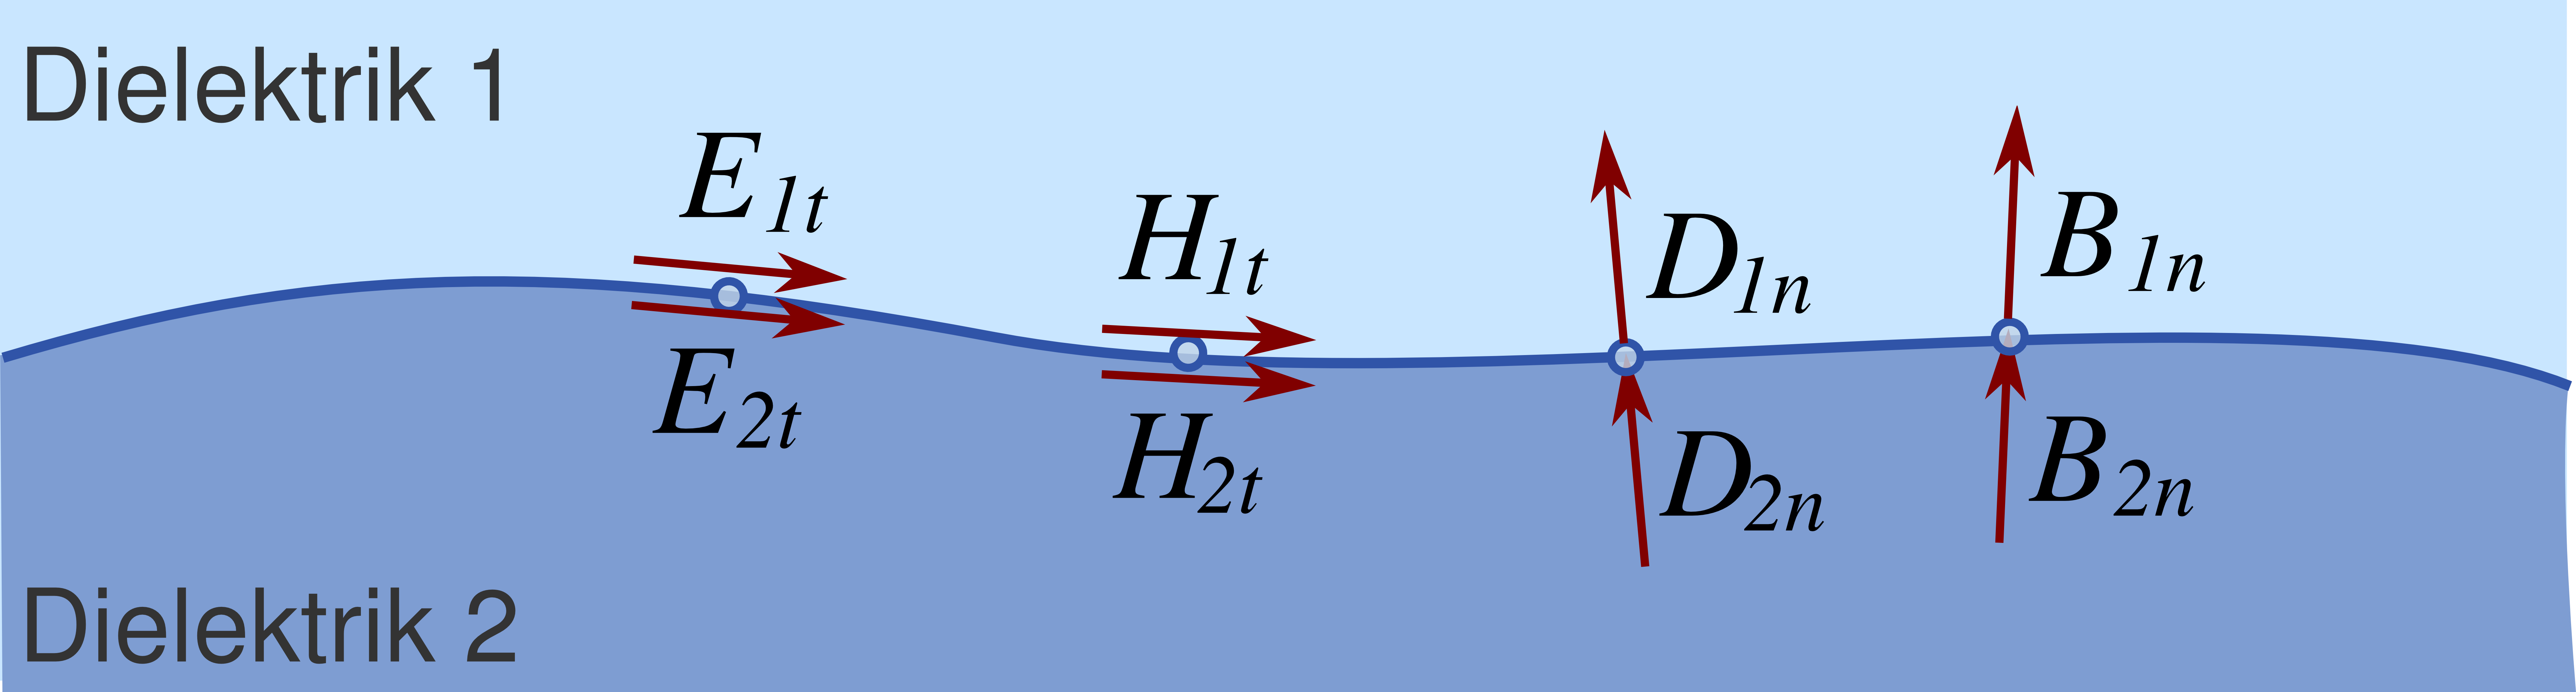
\includegraphics[width=8truecm]{robni_pogoji.png}
\caption{Na meji med dvema dielektrikoma brez površinskih tokov
in nabojev so tangentna
komponenta jakosti električnega in magnetnega polja ter normalna komponenta
gostote magnetnega in električnega polja zvezne količine.}
\label{fig:Robni-pogoji}
\end{figure}


\section{Valovna enačba in Poyntingov vektor}

Večinoma bomo obravnavali elektromagnetna valovanja v izotropnih, 
homogenih in linearnih snoveh brez zunanjih izvorov in
nosilcev naboja ($\mathbf{j}_e=0$ in $\rho_{e}=0$). 
Iz Maxwellovih enačb (\ref{eq:Maxwell1} - \ref{eq:Maxwell4}) izpeljemo valovno 
enačbo\index{Valovna enačba},
ki jo zapišemo za jakost električnega ali magnetnega polja 
\boxeq{eq:valovna-skalarna}{
\nabla^{2}\mathbf{E}-\frac{1}{c^{2}}\frac{\partial^{2}\mathbf{E}}{\partial t^{2}} & = 0\\
\nabla^{2}\mathbf{H}-\frac{1}{c^{2}}\frac{\partial^{2}\mathbf{H}}{\partial t^{2}} & = 0.
}
Pri tem je hitrost valovanja v snovi enaka 
\beq
c=\frac{1}{\sqrt{\epsilon_{0}\epsilon\mu_{0}\mu}}=\frac{c_{0}}{n}.
\eeq
Magnetne in dielektrične lastnosti snovi smo pospravili
v lomni količnik\index{Lomni količnik} 
\beq
n=\frac{c_{0}}{c}=\sqrt{\epsilon\mu}.
\eeq
Za izotropno in nemagnetno snov ($\mu=1$) je lomni količnik $n=\sqrt{\epsilon}$.

\noindent
Vpeljimo še vektor gostote energijskega toka, to je Poyntingov\footnote{Angleški 
fizik John Henry Poynting, 1852-1914.} vektor
\index{Poyntingov vektor}{$\mathbf{S}$}
\beq
\mathbf{S} = \mathbf{E} \times \mathbf{H}.
\label{eq:Poyntingov-vektor}
\eeq
Kot vidimo, je smer energijskega toka vedno pravokotna na smeri $\mathbf{E}$
in $\mathbf{H}$. Gostoto energijskega toka $j$, to je količino
energije, ki v danem časovnem intervalu preteče skozi dano ploskev
z normalo $\mathbf{\hat{n}}$, izračunamo kot časovno povprečje projekcije
Poyntingovega vektorja \index{Intenziteta!elektromagnetno valovanje}
\beq
j=\left\langle \mathbf{\mathbf{S}}\cdot\mathbf{\hat{n}}\right\rangle.
\eeq

\begin{definition}[Poyntingov teorem]
Iz Maxwellovih enačb izpelji kontinuitetno enačbo 
\beq
\nabla\cdot\mathbf{\mathbf{S}}=-\frac{\partial}{\partial t}\left(\frac{1}{2}\epsilon_{0}\mathbf{E}^{2}+
\frac{1}{2}\mu_{0}\mathbf{H}^{2}\right)+\mathbf{E}\cdot\frac{\partial\mathbf{P}}{\partial t}+
\mu_{0}\mathbf{H}\cdot\frac{\partial\mathbf{M}}{\partial t}.
\eeq
Pomagaj si z zvezo $\nabla\cdot(\mathbf{E}\times\mathbf{H})=(\nabla\times\mathbf{E})\cdot\mathbf{H}-
(\nabla\times\mathbf{H})\cdot\mathbf{E}$.
\end{definition}

\noindent
\index{Poyntingov teorem}Opazimo, da predstavlja Poyntingov teorem
izrek o ohranitvi energije. Prvi in drugi člen na desni strani gornje
enačbe opišeta gostoto energije, shranjene v električnem in magnetnem
polju, medtem ko tretji in četrti člen opišeta energijo,
ki je shranjena v snovi (električnih in magnetnih dipolih). Za valovanje
v homogeni izotropni snovi tako velja
\beq
\nabla\cdot\mathbf{S}=-\frac{\partial w}{\partial t},
\eeq
kjer je $w$ \index{Gostota elektromagnetne energije} celotna
gostota energije elektromagnetnega polja. Zapišemo jo kot 
\beq
w=\frac{1}{2}\epsilon_{0}\epsilon\mathbf{E}^{2}+\frac{1}{2}\mu_{0}\mu\mathbf{H}^{2}.
\eeq

\noindent
Valovno enačbo in ohranitvene zakone lahko zapišemo tudi za anizotropne,
nehomogene ali nelinearne snovi. Nekaj teh primerov bomo srečali v nadaljevanju
in jih bomo obravnavali sproti.


\section{Monokromatski elektromagnetni val}

Reševanje valovne enačbe si navadno poenostavimo z uvedbo kompleksnega
zapisa jakosti električnega in magnetnega polja. Račun si
oglejmo na primeru monokromatskega elektromagnetnega vala. Nastavek
za monokromatski val s krožno frekvenco $\omega$ naj bo\index{Elektromagnetno valovanje}
\beq
\mathbf{E}(\mathbf{r},t)  =\mathfrak{\Re}(\mathbf{E}(\mathbf{r})e^{-i\omega t})\qquad \textrm{in} \qquad
\mathbf{H}(\mathbf{r},t)  =\mathfrak{\Re}(\mathbf{H}(\mathbf{r})e^{-i\omega t}),
\eeq
kjer sta $\mathbf E(\mathbf{r})$ in $\mathbf H(\mathbf{r})$ časovno
neodvisna vektorja jakosti električnega in magnetnega polja s kompleksno
amplitudo. Podobno lahko vpeljemo tudi kompleksne vektorje $\mathbf{P}$,
$\mathbf{M}$, $\mathbf{D}$ in $\mathbf{B},$ ki opisujejo realne količine (polarizacijo,
magnetizacijo, gostoto električnega in gostoto magnetnega polja).
V nadaljevanju bomo večinoma pisali polja v kompleksni obliki, pri
čemer se bomo držali gornje definicije. Zavedati pa se moramo, da
je uporaba kompleksnega zapisa zgolj računski pripomoček, na koncu
je treba rezultate vedno izraziti z realnimi količinami. \\

\noindent
Če vstavimo gornji nastavek za monokromatski val v valovno enačbo
(\ref{eq:valovna-skalarna}), dobimo \index{Helmholtzova enačba}Helmholtzovi
enačbi\footnote{Nemški zdravnik in fizik Hermann Ludwig Ferdinand von Helmholtz, 1821-1894.} 
za kompleksna vektorja jakosti električnega in magnetnega polja.
V homogenem in izotropnem sredstvu ju zapišemo kot
\begin{eqnarray}
\nabla^{2}\mathbf{E}(\mathbf{r})+k^{2}\mathbf{E}(\mathbf{r}) & = & 0\label{eq:Helmholtz}\\
\nabla^{2}\mathbf{H}(\mathbf{r})+k^{2}\mathbf{H}(\mathbf{r}) & = & 0,
\end{eqnarray}
kjer je $k=nk_{0}=n\omega/c_{0}$ velikost valovnega vektorja oziroma
valovno število. \newpage

\noindent
Vpeljimo še kompleksni Poyntingov vektor 
\beq
\mathbf{S}(\mathbf{r})=\frac{1}{2}\mathbf{E}\times\mathbf{H}^{*}.\label{eq:Poyntingov-vektor-c}
\eeq

\begin{definition}
Upoštevajoč izraz za Poyntingov vektor $\mathbf{S}$
(enačba \ref{eq:Poyntingov-vektor}) pokaži, da lahko povprečje projekcije Poyntingovega vektorja 
(intenziteto valovanja) $j$ \index{Intenziteta!elektromagnetno valovanje} izrazimo
s kompleksnim Poyntingovim vektorjem $S$ (enačba \ref{eq:Poyntingov-vektor-c}):
\beq
j=\left\langle \mathbf{\mathbf{S}}\cdot\mathbf{\hat{n}}\right\rangle =
\frac{1}{4}\left(\mathbf{E}\times\mathbf{H}^{*}+\mathbf{E}^{*}\times\mathbf{H}\right)=\Re(\mathbf{S}).
\eeq
\end{definition}


\section{Ravni val}

Osnovna rešitev valovne enačbe je ravni val. Nastavek, ki predstavlja
ravni val in hkrati reši Helmholtzovo enačbo (\ref{eq:Helmholtz}), je 
\begin{align}
\mathbf{E}(\mathbf{r},t) & =\mathbf{E}(\mathbf{r})e^{-i\omega t}=
\mathbf{E}_{0}e^{i\mathbf{k}\cdot\mathbf{r}-i \omega t}\\
\mathbf{H}(\mathbf{r},t) & =\mathbf{H}(\mathbf{r})e^{-i\omega t}=
\mathbf{H}_{0}e^{i\mathbf{k}\cdot\mathbf{r}-i \omega t},
\end{align}
pri čemer sta vektorja $\mathbf{E}_{0}$ ter $\mathbf{H}_{0}$ krajevno in časovno
neodvisna. Velikost valovnega vektorja $\mathbf{k}$ je $k=nk_{0},$ pri
čemer je $n$ lomni količnik izotropne in homogene snovi. \\

\noindent
Vektorja jakosti električnega in magnetnega polja zadostujeta
Maxwellovim enačbam (\ref{eq:Maxwell1} - \ref{eq:Maxwell4}), iz česar sledi 
(glej nalogo \ref{naloga-TEM-ortogonalnost}), da sta polji vedno medsebojno pravokotni, 
hkrati pa pravokotni na valovni vektor $\mathbf{k}$. Tak val zato imenujemo transverzalni elektromagnetni
val.\index{Elektromagnetno valovanje!transverzalno valovanje (TEM)}. 

\begin{definition}\label{naloga-TEM-ortogonalnost}
Pokaži, da je za ravni val vedno velja $\mathbf{D} \perp \mathbf{k}$ in 
$\mathbf{B} \perp \mathbf{k}$. Izpelji še pravokotnost polj in valovnega vektorja
v izotropni snovi 
\begin{align}
\mathbf{k}\times\mathbf{H}_{0} & =-\omega\epsilon\epsilon_{0}\mathbf{E}_{0}\label{eq:TEM-pogoj1}\\
\mathbf{k}\times\mathbf{E}_{0} & =\omega\mu\mu_{0}\mathbf{H}_{0}.\label{eq:TEM-pogoj2}
\end{align}
\end{definition}

\noindent
Zaradi enolične zveze med električnim in magnetnim poljem zadošča
za opis ravnega vala le eno polje, navadno se odločimo za električno.
\\

\noindent
Energijski tok je pri ravnem valu v izotropni snovi vedno v smeri valovnega vektorja, pravokotno
na valovne fronte. Iz definicije za gostoto svetlobnega toka (\ref{eq:Poyntingov-vektor-c})
in Maxwelovih enačb sledi\index{Intenziteta!ravni val}
\beq
j=\Re\left(\frac{1}{2}E_{0}H_{0}^{*}\right)=
\frac{1}{2}c\epsilon\epsilon_{0}\left|E_{0}\right|^{2}=\frac{1}{2}c_{0}n\epsilon_{0}\left|E_{0}\right|^{2}.
\eeq
Gostota svetlobnega toka (intenziteta svetlobe) je torej sorazmerna
s kvadratom amplitude jakosti električnega polja. Gostoti toka $j=1~\mathrm{kW/m^{2}}$
tako v praznem prostoru ustreza jakost električnega polja
$E_{0}=868~\mathrm{V/m}$, gostoti $j=1~\mathrm{W/\mu m^{2}}$ pa 
$E_{0}=27~\mathrm{MV/m}$. \\

\noindent
Zapišimo še povprečno gostoto energije valovanja. K energiji prispevata
tako magnetno kot električno polje. Oba prispevka sta enaka, zato velja
\beq
\left\langle w\right\rangle =\frac{1}{4}\epsilon\epsilon_{0}\left|E_{0}\right|^{2}+
\frac{1}{4}\mu\mu_{0}\left|H_{0}\right|^{2}=\frac{1}{2}\epsilon\epsilon_{0}\left|E_{0}\right|^{2}.
\eeq
Povprečna gostota energije $w$, pomnožena s hitrostjo svetlobe v
snovi, da gostoto energijskega toka $j$ oziroma intenziteto svetlobe
\boxeq{eq:jcw}{
j=cw.
}
Gornji izraz nazorno kaže, da je intenziteta svetlobe pravzaprav pretok
energije. To si lahko predstavljamo, če vzamemo valj s prečnim presekom
$S$ in volumnom $Sc\Delta t$, v katerem je shranjene $wSc\Delta t$
energije. Energija, ki preteče skozi presek $S$ v času $\Delta t$,
je ravno $cw$. \\

\noindent
Intenziteta ravnega vala je neodvisna od kraja in časa, iz česar sledi,
da je povsod po prostoru enaka. Če bi hoteli izračunati energijo,
ki jo nosi ravni val, bi opazili, da je ta energija neskončna. To
seveda ni mogoče, zato se je vedno treba zavedati, da je ravni val
le idealiziran, a nazoren in praktičen približek elektromagnetnega
vala.


\section{Polarizacija EM valovanja}

Jakost električnega polja elektromagnetnega valovanja je v izotropnem
sredstvu pravokotna na smer valovnega vektorja\footnote{V splošnem je
jakost električnega polja pravokotna na smer Poyntingovega vektorja ($\mathbf{E}\perp\mathbf{S}$) in 
gostota električnega polja pravokotna na smer valovnega vektorja ($\mathbf{D}\perp\mathbf{k}$). 
V anizotropnih sredstvih velja namreč $\mathbf k\nparallel\mathbf S$.}. Vektor $\mathbf{E}$
torej leži v ravnini, pravokotni na smer valovnega vektorja, njegovo
smer pa opiše polarizacija. \\

\noindent
V splošnem je ravni val eliptično polariziran. Takrat vektor $\mathbf E$
v ravnini, pravokotni na valovni vektor, oriše elipso. Obe komponenti vektorja 
$\mathbf{E}(\mathbf{r})$ nihata sinusno z enako frekvenco, lahko pa se razlikujeta
amplituda in faza. Kadar je elipsa izrojena v daljico, dobimo linearno polarizirano valovanje,
kadar pa je krog, dobimo cirkularno polariziran val. Poljubno polarizacijo
lahko vedno zapišemo kot vsoto dveh linearno ali dveh cirkularno polariziranih
valovanj. \\

\noindent
Polarizacijo valovanja lahko zapišemo s kompleksnim \index{Jonesov vektor}Jonesovim 
vektorjem\footnote{Ameriški fizik Robert Clark Jones, 1916-2004.}
$\mathbf{J}$. Za monokromatski ravni val, ki se širi v smeri $z$, je 
\beq
\mathbf{J}=\frac{1}{|E_{0}|}\left[\begin{array}{c}
E_{x}\\
E_{y}
\end{array}\right].
\eeq
Dodali smo normalizacijski faktor $|E_{0}|=\sqrt{|E_{x}|^{2}+|E_{y}|^{2}}$,
da je Jonesov vektor normaliziran in $\mathbf{J}\cdot\mathbf{J}^{*}=1$.
Ravni val, linearno polariziran v smeri $x$, tako zapišemo kot $\mathbf{J}=\left(1,0\right)$,
val, ki je linearno polariziran pod kotom $45^{\circ}$ glede na osi
$x$ in $y$, pa je $\mathbf{J}=\frac{1}{\sqrt{2}}\left(1,1\right)$.
Desno cirkularno polarizirano valovanje predstavlja vektor $\mathbf{J}=\frac{1}{\sqrt{2}}\left(1,-i\right)$,
levo cirkularno polarizirano pa $\mathbf{J}=\frac{1}{\sqrt{2}}\left(1,i\right)$.
Desno polariziran val je torej tisti val, pri katerem se električna
poljska jakost na danem mestu vrti v desno, če gledamo v smeri širjenja
valovanja. Hkrati pa velja, da električna poljska jakost ob danem
času vzdolž smeri širjenja valovanja opiše levosučno vijačnico. \\

\noindent
Zapis z Jonesovim vektorjem je prikladen, saj omogoča preprost izračun
prehoda ravnega vala skozi optične elemente, ki spreminjajo polarizacijo,
a ohranjajo obliko ravnega vala. V splošnem se pri prehodu skozi
sredstvo spremeni kompleksna amplituda $\mathbf{E}_1 = (E_{1x},E_{1y})$ 
\begin{align}
E_{2x} & =T_{11}E_{1x}+T_{12}E_{1y}\\
E_{2y} & =T_{21}E_{1x}+T_{22}E_{1y},
\end{align}
pri čemer so komponente $T_{ij}$ odvisne od lastnosti sredstva. Gornji
enačbi lahko strnjeno zapišemo v matrični obliki
\beq
\mathbf{J}_{2}=T\cdot\mathbf{J}_{1},
\eeq
kjer sta $\mathbf{J}_{1}=(E_{1x},E_{1y})$ in $\mathbf{J}_{2}=(E_{2x},E_{2y})$
vstopni in izstopni val, $T$ pa je \index{Jonesova matrika}Jonesova
matrika. Jonesova matrika za prehod skozi linearni polarizator, ki
polarizira v smeri $x$, je
\beq
T=\left[\begin{array}{cc}
1 & 0\\
0 & 0
\end{array}\right].
\eeq
Oglejmo si še dva zanimiva primera optičnih komponent, to sta $\lambda/2$
in $\lambda/4$ ploščici. Jonesova matrika za $\lambda/2$ ploščico
je
\beq
T=\left[\begin{array}{cc}
1 & 0\\
0 & -1
\end{array}\right].
\eeq
Kratek račun pokaže, da $\lambda/2$ ploščica spremeni desno cirkularno
polarizariziran val v levo polariziran in obratno. Jonesova matrika
za $\lambda/4$ ploščico je 
\beq
T=\left[\begin{array}{cc}
1 & 0\\
0 & i
\end{array}\right].
\eeq
Ta optični element linerno polarizirano valovanje oblike $\frac{E_{0}}{\sqrt{2}}(1,1)$
spremeni v levo cirkularno polarizirano valovanje, cirkularno polarizirano
valovanje pa nazaj v linearno. 

\begin{definition}
Pokaži, da je Jonesova matrika za polarizator,
ki prepušča polarizacijo pod kotom $\vartheta$ glede na os $x$, podana z
\beq
T=\left[\begin{array}{cc}
\cos^{2}\vartheta & \sin\vartheta\cos\vartheta\\
\sin\vartheta\cos\vartheta & \sin^{2}\vartheta
\end{array}\right].
\eeq
Namig: matriko $T'$, ki predstavlja polarizator v smeri $x$, zapiši v zavrtenem
koordinatnem sistemu $T=R(\vartheta)^\textrm{T} \cdot {T'}\cdot R(\vartheta)$, kjer je $R(\vartheta)$ rotacijska 
matrika.
\end{definition}


\section{Lom in odboj EM valovanja}

Na ravni meji med dvema izotropnima dielektrikoma se del svetlobe
odbije po odbojnem zakonu, del pa lomi po lomnem zakonu
\beq
n_{1}\sin\vartheta_{1}=n_{2}\sin\vartheta_{2}.
\label{eq:lomni_zakon}
\eeq
S kotoma $\vartheta_{1}$in $\vartheta_{2}$ smo označili vpadni in lomni
kot, $n_{1}$in $n_{2}$ pa sta lomna količnika prve in druge snovi.
Poglejmo, kaj se pri lomu in odboju zgodi s polarizacijo valovanja.
Os $x$ vpadnega vala naj bo pravokotna na vpadno ravnino (slika~\ref{fig:Lom}). 
Valovanje, polarizirano v tej smeri, je transverzalno električno
(TE) valovanje. Takrat je električna poljska jakost vzporedna mejni ravnini. 
Kadar leži v mejni ravnini jakost magnetnega polja, gre za transverzalno 
magnetno valovanje (TM).
\begin{figure}[h]
\centering
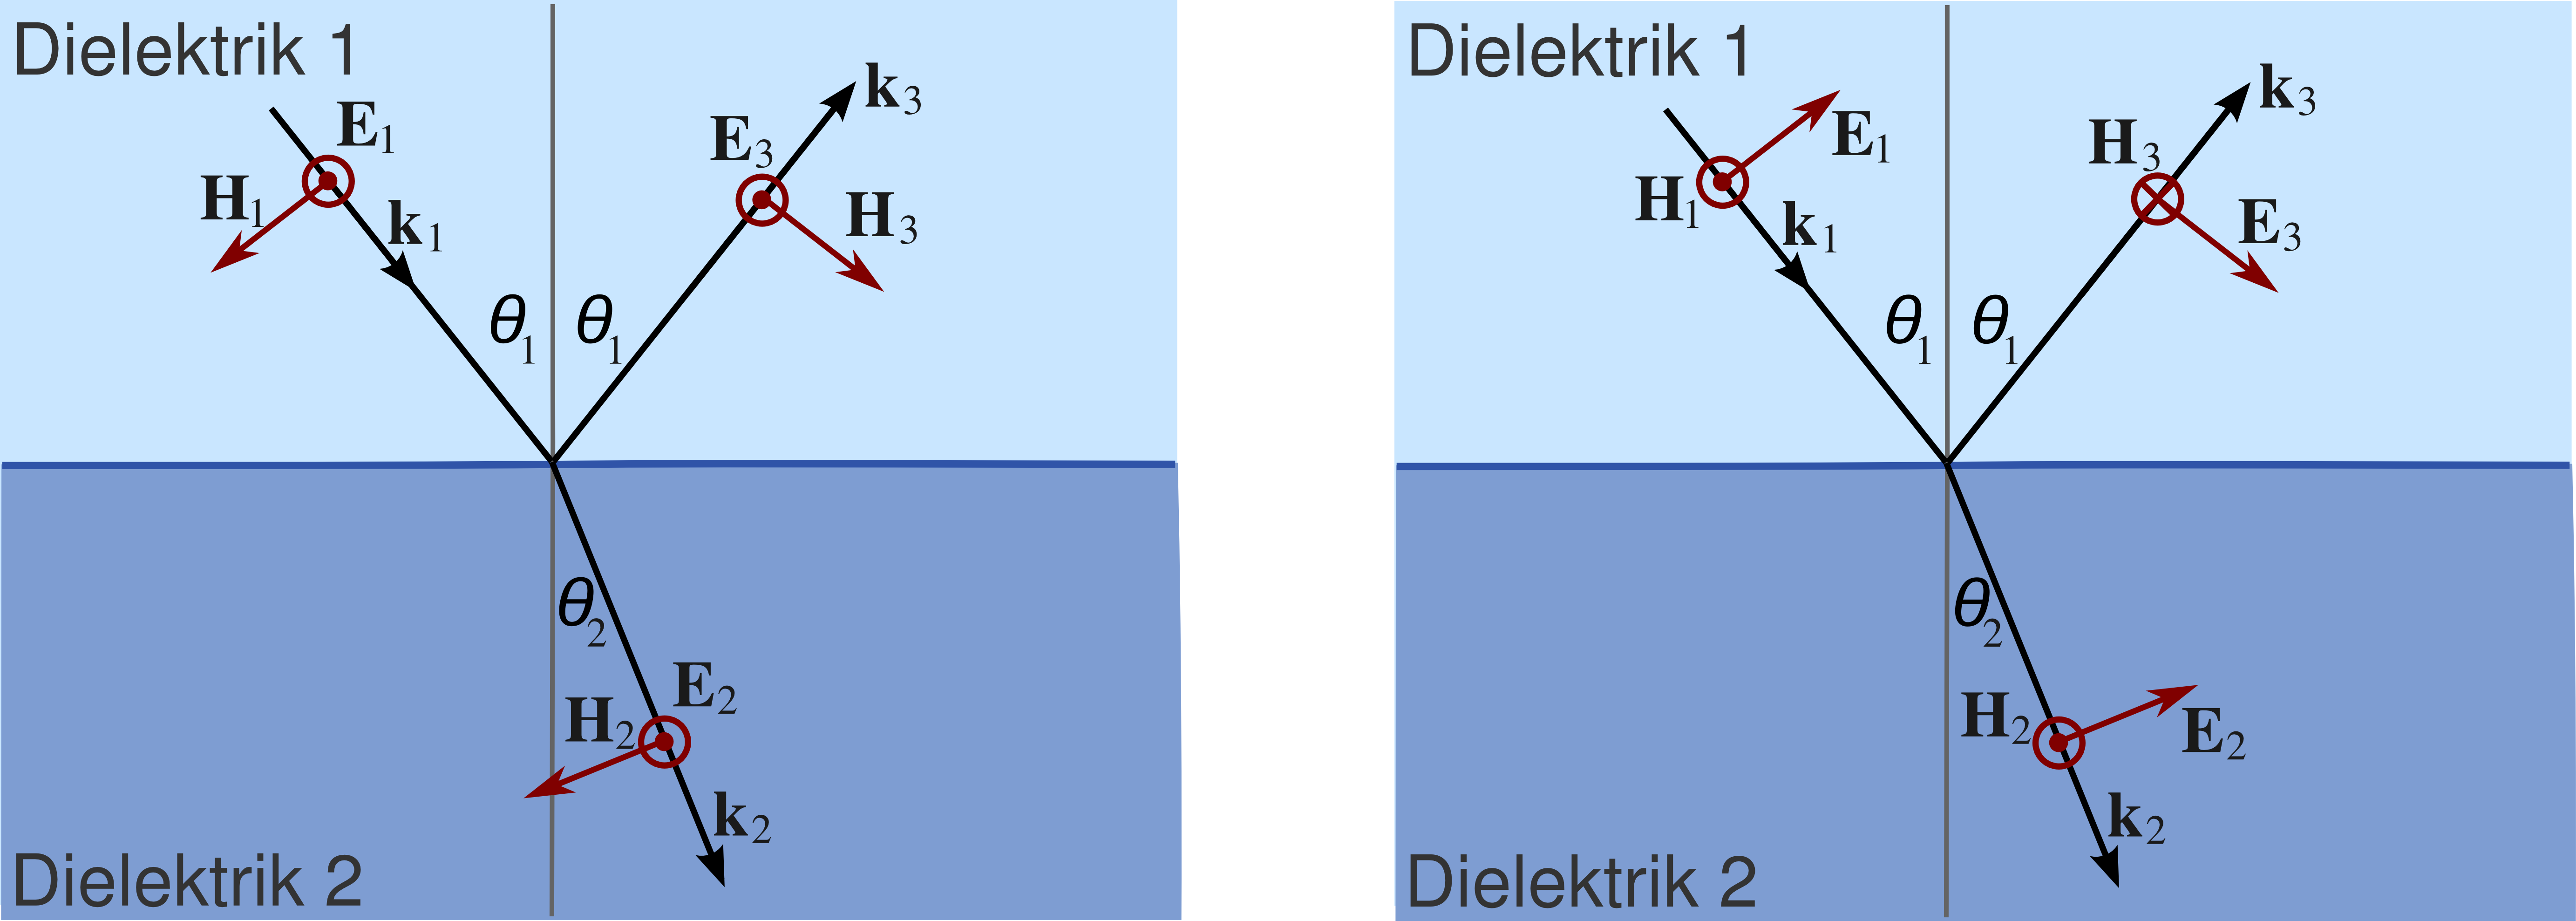
\includegraphics[width=12truecm]{lom.png}
\caption{Lom elektromagnetnega valovanja. Levo: transverzalno električno (TE) valovanje. 
Desno: transverzalno magnetno (TM) valovanje. Os $x$ je pravokotna na vpadno ravnino 
in kaže iz lista.}
\label{fig:Lom}
\end{figure}
\\

\noindent
Jonesovi matriki za odbojnost $r$ in prepustnost $t$
na plasti med dvema dielektrikoma zapišemo kot 
\beq
r=\left[\begin{array}{cc}
r_{x} & 0\\
0 & r_{y}
\end{array}\right] \qquad \textrm{in} \qquad t=\left[\begin{array}{cc}
t_{x} & 0\\
0 & t_{y}
\end{array}\right].
\eeq

\noindent
Potem je 
\begin{align}
E_{2x} & =t_{x}E_{1x} \qquad \qquad E_{3x} =r_{x}E_{1x}\\
E_{2y} & =t_{y}E_{1y} \qquad \qquad E_{3y}=r_{y}E_{1y},
\end{align}
pri čemer smo z $\mathbf{E}_{2}$ označili prepuščeni val, z $\mathbf{E}_{3}$ pa odbitega.
Iz robnih pogojev (\ref{eq:robni-pogoji}) izračunamo koeficiente matrik
$r$ in $t$ s \index{Fresnelove enačbe}Fresnelovimi 
enačbami\footnote{Francoski fizik Augustin-Jean Fresnel, 1788-1827.}:
\beq
r_{x}=\frac{n_{1}\cos\vartheta_{1}-n_{2}\cos\vartheta_{2}}{n_{1}\cos\vartheta_{1}+n_{2}\cos\vartheta_{2}},
\qquad t_{x}=1+r_{x}=\frac{2n_{1}\cos\vartheta_{1}}{n_{1}\cos\vartheta_{1}+n_{2}\cos\vartheta_{2}}
\eeq
in
\beq
r_{y}=\frac{n_{1}\cos\vartheta_{2}-n_{2}\cos\vartheta_{1}}{n_{1}\cos\vartheta_{2}+n_{2}\cos\vartheta_{1}},
\qquad t_{y}=(1+r_{y})\frac{\cos\vartheta_{1}}{\cos\vartheta_{2}}=\frac{2n_{1}\cos\vartheta_{1}}
{n_{1}\cos\vartheta_{2}+n_{2}\cos\vartheta_{1}}.
\eeq

\noindent
V splošnem sta odbojnost $r$ in prepustnost $t$ kompleksni
količini, saj iz lomnega zakona sledi, da je $\cos\vartheta_{2}=
\sqrt{1-\left(n_{1}/n_{2}\right)^{2}\sin^{2}\vartheta_{1}}$
lahko kompleksen. Velikost števila $\left|r\right|$ tako predstavlja
odbojnost, argument $\arg\{r\}$ pa spremembo faze
pri odboju.\\

\noindent
Prepustnost $r$ in odbojnost $t$ povesta, kako se spremeni kompleksna
amplituda jakosti električnega polja. Razmerje med intenziteto odbite
in vpadne svetlobe $\mathcal{R}$ oziroma razmerje med intenziteto prepuščene in vpadne svetlobe
$\mathcal{T}$ pa izračunamo kot 
\beq
\mathcal{R}=\left|r\right|^{2}
\eeq
in
\beq
\mathcal{T}=1-\mathcal{R}.
\eeq
Slednja enačba sledi iz ohranitve energije. V splošnem $\mathcal{T}$
ni enak $\left|t\right|^{2},$ saj energijski tok potuje po različnih
snoveh in v različnih smereh. Velja zveza
\beq
\mathcal{T}=\frac{n_{2}\cos\vartheta_{2}}{n_{1}\cos\vartheta_{1}}\left|t\right|^{2}.
\eeq


\begin{definition}
Pokaži, da za TM val obstoja vpadni kot
\beq
\vartheta_{B}=\arctan\left(\frac{n_2}{n_1}\right),
\eeq
pri katerem je odbojnost enaka nič oziroma prepustnost enaka $\mathcal{T}=$1.
Ta kot imenujemo \index{Brewsterjev kot}Brewsterjev 
kot. Brewsterjeva
okna (steklene ploščice, postavljene pod Brewsterjevim kotom) uporabljamo
v resonatorjih laserjev za povečanje izgub TE in zmanjšanje izgub
TM polariziranega valovanja.
\end{definition}

\noindent
Pri prehodu skozi optične elemente (leče, polarizatorje ...) se -
razen TM polariziranega valovanja pri Brewsterjevem 
kotu\footnote{Škotski fizik in znanstvenik Sir David Brewster, 1781-1868.} - vedno nekaj
svetlobe odbije. Da zmanjšamo te izgube, optične elemente navadno
prekrijemo z antirefleksno plastjo, to je nanosom ene ali več primerno
izbranih debelin plasti dielektrikov z ustreznimi lomnimi količniki.
Zaradi destruktivne interference se količina odbite svetlobe z izbrano
valovno dolžino občutno zmanjša. Ker imamo v fiziki laserjev opraviti
s koherentnimi izvori s točno določeno valovno dolžino, za zmanjšanje
izgub, na primer v resonatorju laserja, vedno uporabljamo optične
elemente (leče, kristale, akustooptične modulatorje ... ) z ustrezno
antirefleksno plastjo.

\section{EM valovanje v anizotropnih snoveh}

Do zdaj smo obravnavali elektromagnetno valovanje
v izotropnih snoveh, v katerih je dielektričnost skalar in hitrost širjenja
valovanja neodvisna od njegove smeri. V splošnem pa so snovi anizotropne,
dielektričnost je tenzor, hitrost potovanja svetlobe skozi snov pa
je odvisna od smeri razširjanja in od polarizacije valovanja. \\

\noindent
Gostoto električnega polja v anizotropni snovi zapišemo kot 
\beq
\mathbf{D}=\epsilon_{0}\underline{\epsilon} \cdot\mathbf{E} = 
\epsilon_{0}
\left[\begin{array}{ccc}
\epsilon_{11} & \epsilon_{12}& \epsilon_{13}\\
\epsilon_{21} & \epsilon_{22}& \epsilon_{23}\\
\epsilon_{31} & \epsilon_{32}& \epsilon_{33}\\
\end{array}\right]\mathbf{E},
\label{eq:gostota-elektricnega-polja-tenzor}
\eeq
kjer je $\epsilon_{ij}$ tenzor drugega reda in ima v splošnem devet komponent.
V dielektričnih snoveh, v katerih ne pride do optične aktivnosti ali absorbcije, je tenzor
realen in simetričen $\epsilon_{ij}=\epsilon_{ji}$. Tak tenzor lahko vedno
diagonaliziramo, torej poiščemo koordinatni sistem, v katerem je tenzor $\underline{\epsilon}$
diagonalen. V takem koordinatnem sistemu velja 
\beq
\mathbf{D} = \epsilon_{0}
\left[\begin{array}{ccc}
\epsilon_{1} & 0& 0\\
0 & \epsilon_{2}& 0\\
0 & 0& \epsilon_{3}\\
\end{array}\right]\mathbf{E}
\eeq
in 
\beq
D_{1}=\epsilon_{0}\epsilon_{1}E_{1},\quad D_{2}=\epsilon_{0}\epsilon_{2}E_{2},\quad D_{3}=\epsilon_{0}\epsilon_{3}E_{3}.\label{eq:gostota-elektricnega-polja-lastni}
\eeq
Glavne osi sistema torej določajo smeri, vzdolž katerih sta jakost
in gostota električnega polja vzporedni, lastne vrednosti 
pa ustrezajo trem lomnim količnikom $\epsilon_{i}=\sqrt{n_{i}}$. Kristale,
za katere so vse tri vrednosti $n_i$ različne, imenujemo optično dvoosni kristali, medtem 
ko sta v optično enoosnih kristalih dve lastni vrednosti enaki $n_{1}=n_{2}$. 
Če so enake vse tri vrednosti, je snov izotropna.\\

\subsection*{Optična indikatrisa}
Poglejmo, kako se po anizotropnih snoveh širi valovanje v odvisnosti
od njegove smeri in polarizacije. Preprost primer je valovanje, ki se širi vzdolž lastne
osi $z$, polarizirano pa je vzdolž lastne osi $x$. Pri prehodu
skozi kristal se polarizacija valovanja ohrani, lomni količnik za
tak val pa je $n_{1}$. Podobno velja za val, polariziran v smeri
$y$, za katerega je lomni količnik enak $n_{2}$. Če se valovanje širi vzdolž lastne
osi $z$, vendar njegova polarizacija ne sovpada z lastnima osema
$x$ ali $y$, dobimo po prehodu skozi kristal iz vpadnega linearno polariziranega valovanja
v splošnem eliptično valovanje. Lastni komponenti namreč potujeta z različnima
hitrostima, zato pride med njima do faznega zamika.\\
\begin{figure}[h]
\centering
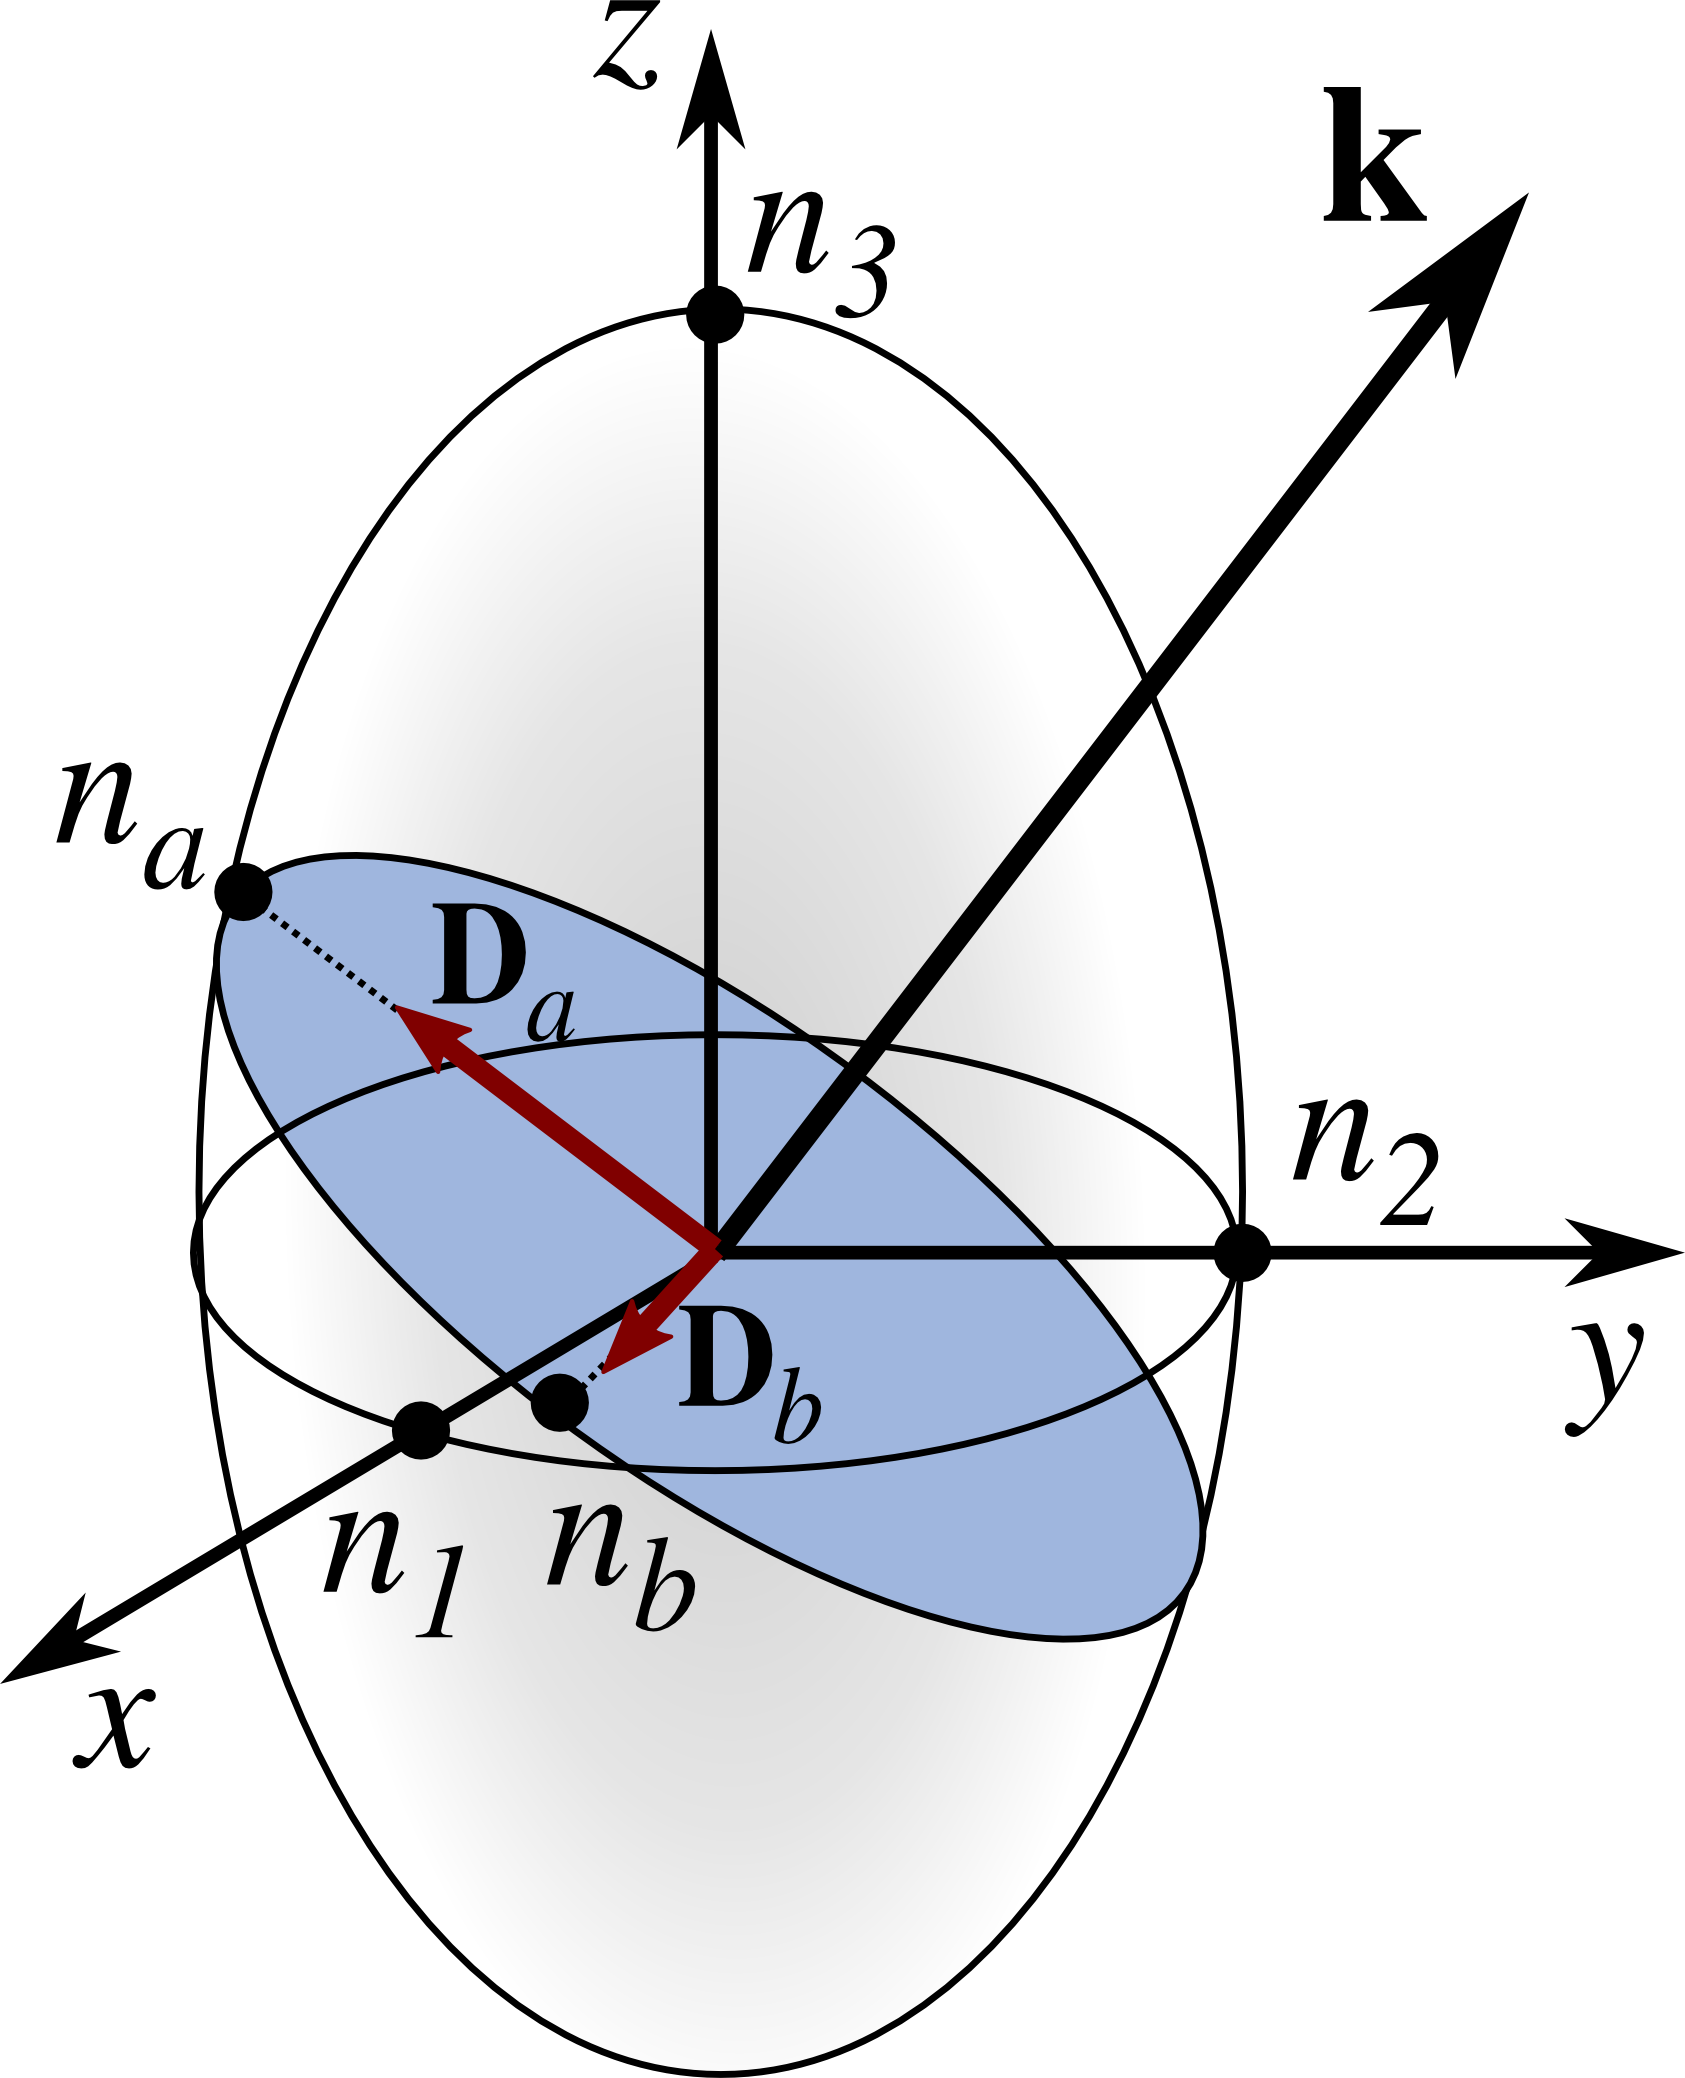
\includegraphics[width=4truecm]{indikatrisa.png}
\caption{\label{fig:Indikatrisa}Optična indikatrisa oziroma elipsoid lomnega količnika. Glavne osi
elipsoida sovpadajo z glavnimi osmi tenzorja $\varepsilon$, polosi elipsoida pa so enake
lomnim količnikom $n_i$. V primeru optično enoosnega kristala je indikatrisa  
rotacijski elipsoid, v primeru izotropne snovi pa je optična indikaktrisa krogla. }
\end{figure}

\noindent
Za poljubno smer širjenja valovanja ter poljubno polarizacijo je račun
bolj zapleten in moramo lomne količnike še izračunati. Pri tem si pomagamo 
z grafično upodobitvijo, s tako imenovano 
\index{Optična indikatrisa}optično indikatriso (elipsoidom lomnega
količnika). Optična indikatrisa je elipsoid, podan z enačbo
\beq
\frac{x^{2}}{n_{1}^{2}}+\frac{y^{2}}{n_{2}^{2}}+\frac{z^{2}}{n_{3}^{2}}=1.
\eeq
Glavne osi elipsoida sovpadajo z glavnimi osmi tenzorja $\epsilon$, 
polosi elipsoida pa so $n_{1}$, $n_{2}$ in $n_{3}$. 
Za val, ki se širi z valovnim vektorjem $\mathbf{k}$, skozi izhodišče
narišemo ravnino, pravokotno na smer valovnega vektorja (slika \ref{fig:Indikatrisa}).
Presečišče ravnine in elipsoida je elipsa, katere glavni osi podata
vrednosti lomnih količnikov $n_{a}$ in $n_{b}$ za obe lastni polarizaciji,
njuni smeri pa predstavljata lastni smeri gostote električnega polja. Ker
sta to lastni osi, smer jakosti električnega polja izračunamo z
enačbo \ref{eq:gostota-elektricnega-polja-lastni}.\\

\subsection*{Optično enoosni kristali}
V optično enoosnih kristalih sta dve lastni vrednosti enaki in indikatrisa je rotacijski 
elipsoid. Po dogovoru izberemo lastne vrednosti tako, da velja $n_{1}=n_{2}\neq n_{3}$. 
Za valovanje, ki se razširja v smeri $z$, sta lomna količnika za obe polarizaciji 
enaka in os $z$ imenujemo \index{Optična os}optična os. Hitrost valovanja, ki
se širi vzdolž optične osi, je torej neodvisna od njegove polarizacije.
Navadno vpeljemo tudi nove oznake: $n_{1}=n_{2}=n_{o}$, ki označuje redni (\textit{ordinary})
lomni količnik, $n_{3}=n_{e}$ pa izredni (\textit{extraordinary}) lomni količnik. 
\begin{figure}[h]
\centering
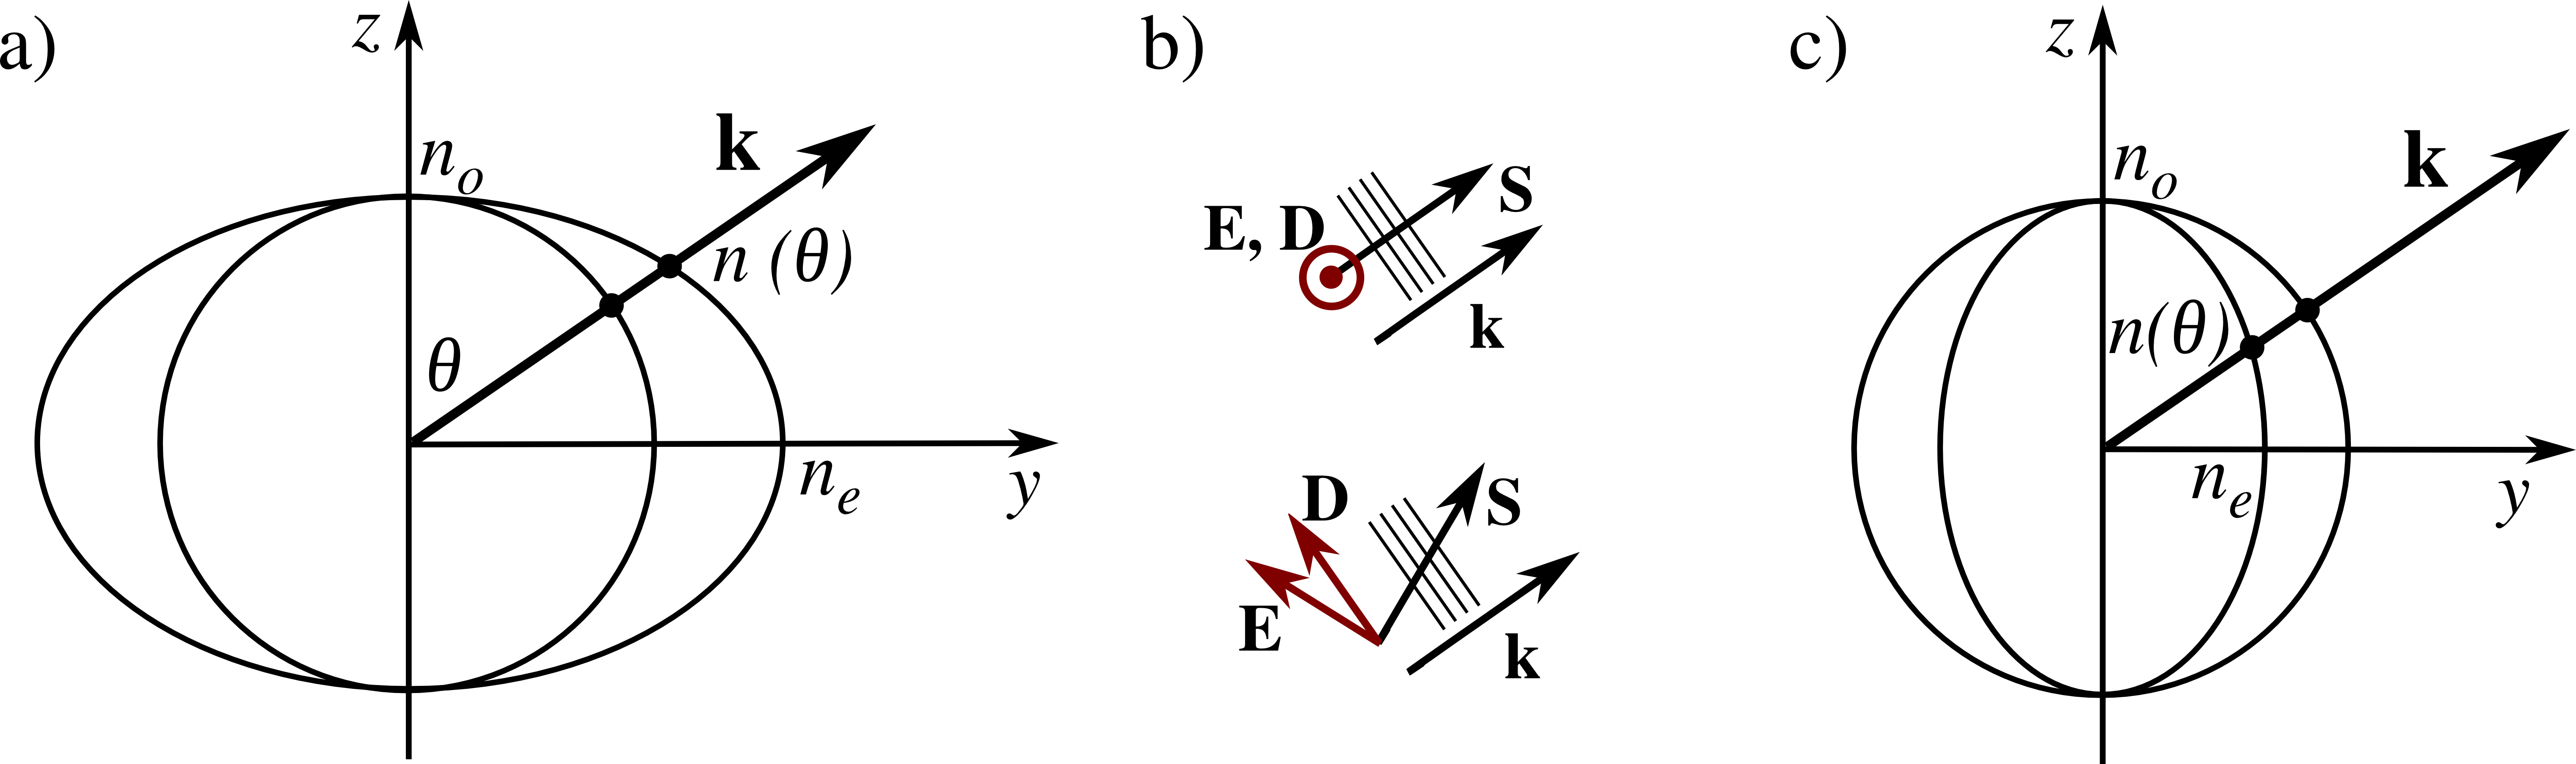
\includegraphics[width=12truecm]{elipsa.png}
\caption{\label{fig:Elipsa}V optično enoosnih kristalih je lomni količinik odvisen
od smeri valovnega vektorja in njegove polarizacije. a) primer pozitivno anizotropne
snovi ($n_e>n_o$). b) Redni žarek je polariziran pravokotno na vpadno ravnino. Zanj velja, 
da je $\mathbf{D} \parallel \mathbf{E}$ in $\mathbf{S} \parallel \mathbf{k}$. Izredni žarek
je polariziran v vpadni ravnini. Smer širjenja žarka $\mathbf{S}$ ni vzporedna z valovnim vektorjem
$\mathbf{k}$,
prav tako valovne fronte niso pravokotne nanjo. c) Primer negativno anizotropne snovi ($n_e< n_o$).}
\end{figure}\\

\noindent
Zaradi simetrije je pri izračunu lomnega količnika pomemben le kot 
$\vartheta$ med valovnim vektorjem $\mathbf{k}$ in optično osjo $z$. Dvema 
lastnima polarizacijama pripadata dva različna lomna količnika. 
Za lažjo predstavo oba lomna količnika skiciramo v odvisnosti
od kota $\vartheta$ (slika~\ref{fig:Elipsa}). Lomni količnik za žarek, ki
je polariziran pravokotno na vpadno ravnino, je neodvisen od $\vartheta$, zato narišemo krog.
Takemu žarku pravimo \index{Redni žarek}redni žarek. 
Žarek, ki je polariziran v vpadni ravnini, je tako imenovan izredni žarek. Pripadajoč
lomni količnik je odvisen od kota $\vartheta$ in ga izračunamo iz sledeče enačbe elipse
s polosema $n_o$ in $n_e$: 
\beq
\frac{1}{n^{2}(\vartheta)}=\frac{\cos^{2}\vartheta}{n_{o}^{2}}+\frac{\sin^{2}\vartheta}{n_{e}^{2}}.
\label{eq:izreden}
\eeq
Opazimo, da se krožnica in elipsa dotikata ravno na osi $z$. Takrat se 
valovanje širi vzdolž optične osi in lomna količnika sta za obe polarizaciji enaka $n_o$. \\

\noindent
Navadno sta pri ravnem valu vektorja $\mathbf{E}$ in $\mathbf{D}$ vzporedna, 
prav tako $\mathbf{k}$ in $\mathbf{S}$. Žarek se širi v smeri valovnega vektorja, 
valovne fronte pa so pravokotne nanj. To velja tudi za redni žarek v anizotropnih
snoveh. Izredni žarek pa ima, kot že ime nakazuje, ``izredne'' lastnosti. Vektorja
$\mathbf{E}$ in $\mathbf{D}$ nista vzporedna, zato tudi valovni vektor $\mathbf{k}$ ni vzporeden
toku energije oziroma Poyntingovemu vektoru $\mathbf{S}$ (slika \ref{fig:Elipsa}b). 
Žarek, ki ga vidimo, torej potuje v smeri, ki ni enaka smeri valovnega vektorja. Smer
Poyntingovega vektorja določimo kot normalo na elipso pri kotu $\vartheta$. 

\subsection*{Dvojni lom}
Ko vpade žarek na anizotropno snov, se lomi. Hitrost valovanja v snovi - in s tem 
tudi kot, pod katerim se lomi - je odvisna od polarizacije valovanja in v splošnem
dobimo dva lomljena žarka z različnima polarizacijama. Da zadostimo ohranitvi faze
pri prehodu med snovema, moramo popraviti tudi lomni zakon (\ref{eq:lomni_zakon}).
Privzemimo še, da je lomni količnik snovi, iz katere valovanje prehaja v anizotropen kristal, enak 1. 
Za redni val s TE polarizacijo potem velja
\beq
\sin\vartheta_{1}=n_{o}\sin\vartheta_{o},
\eeq
za izredni val s TM polarizacijo pa
\beq
\sin\vartheta_{1}=n(\vartheta_e)\sin\vartheta_{e},
\eeq
pri čemer $n(\vartheta_e)$ izračunamo iz (\ref{eq:izreden}).\\

\noindent

Tudi pri pravokotnem vpadu
\textcolor{red}{(samo, če os postrani!)} se izredni žarek lomi v kristalu
ter na izstopni strani kristala se odmakne od rednega žarka. To je
posledica elektromagnetne interakcije med svetlobo in snovjo zato
tega pojava z lomnim zakonom ter žarkovno optiko ne moremo opisati.
Dovolj dolg enoosni kristal odrezan pod primernim kotom lahko tako
služi kot polarizacijski delilnik žarkov, saj sta obe komponenti polarizacije
na izstopni strani kristala prostorsko razmaknjeni. 
\begin{figure}
\centering
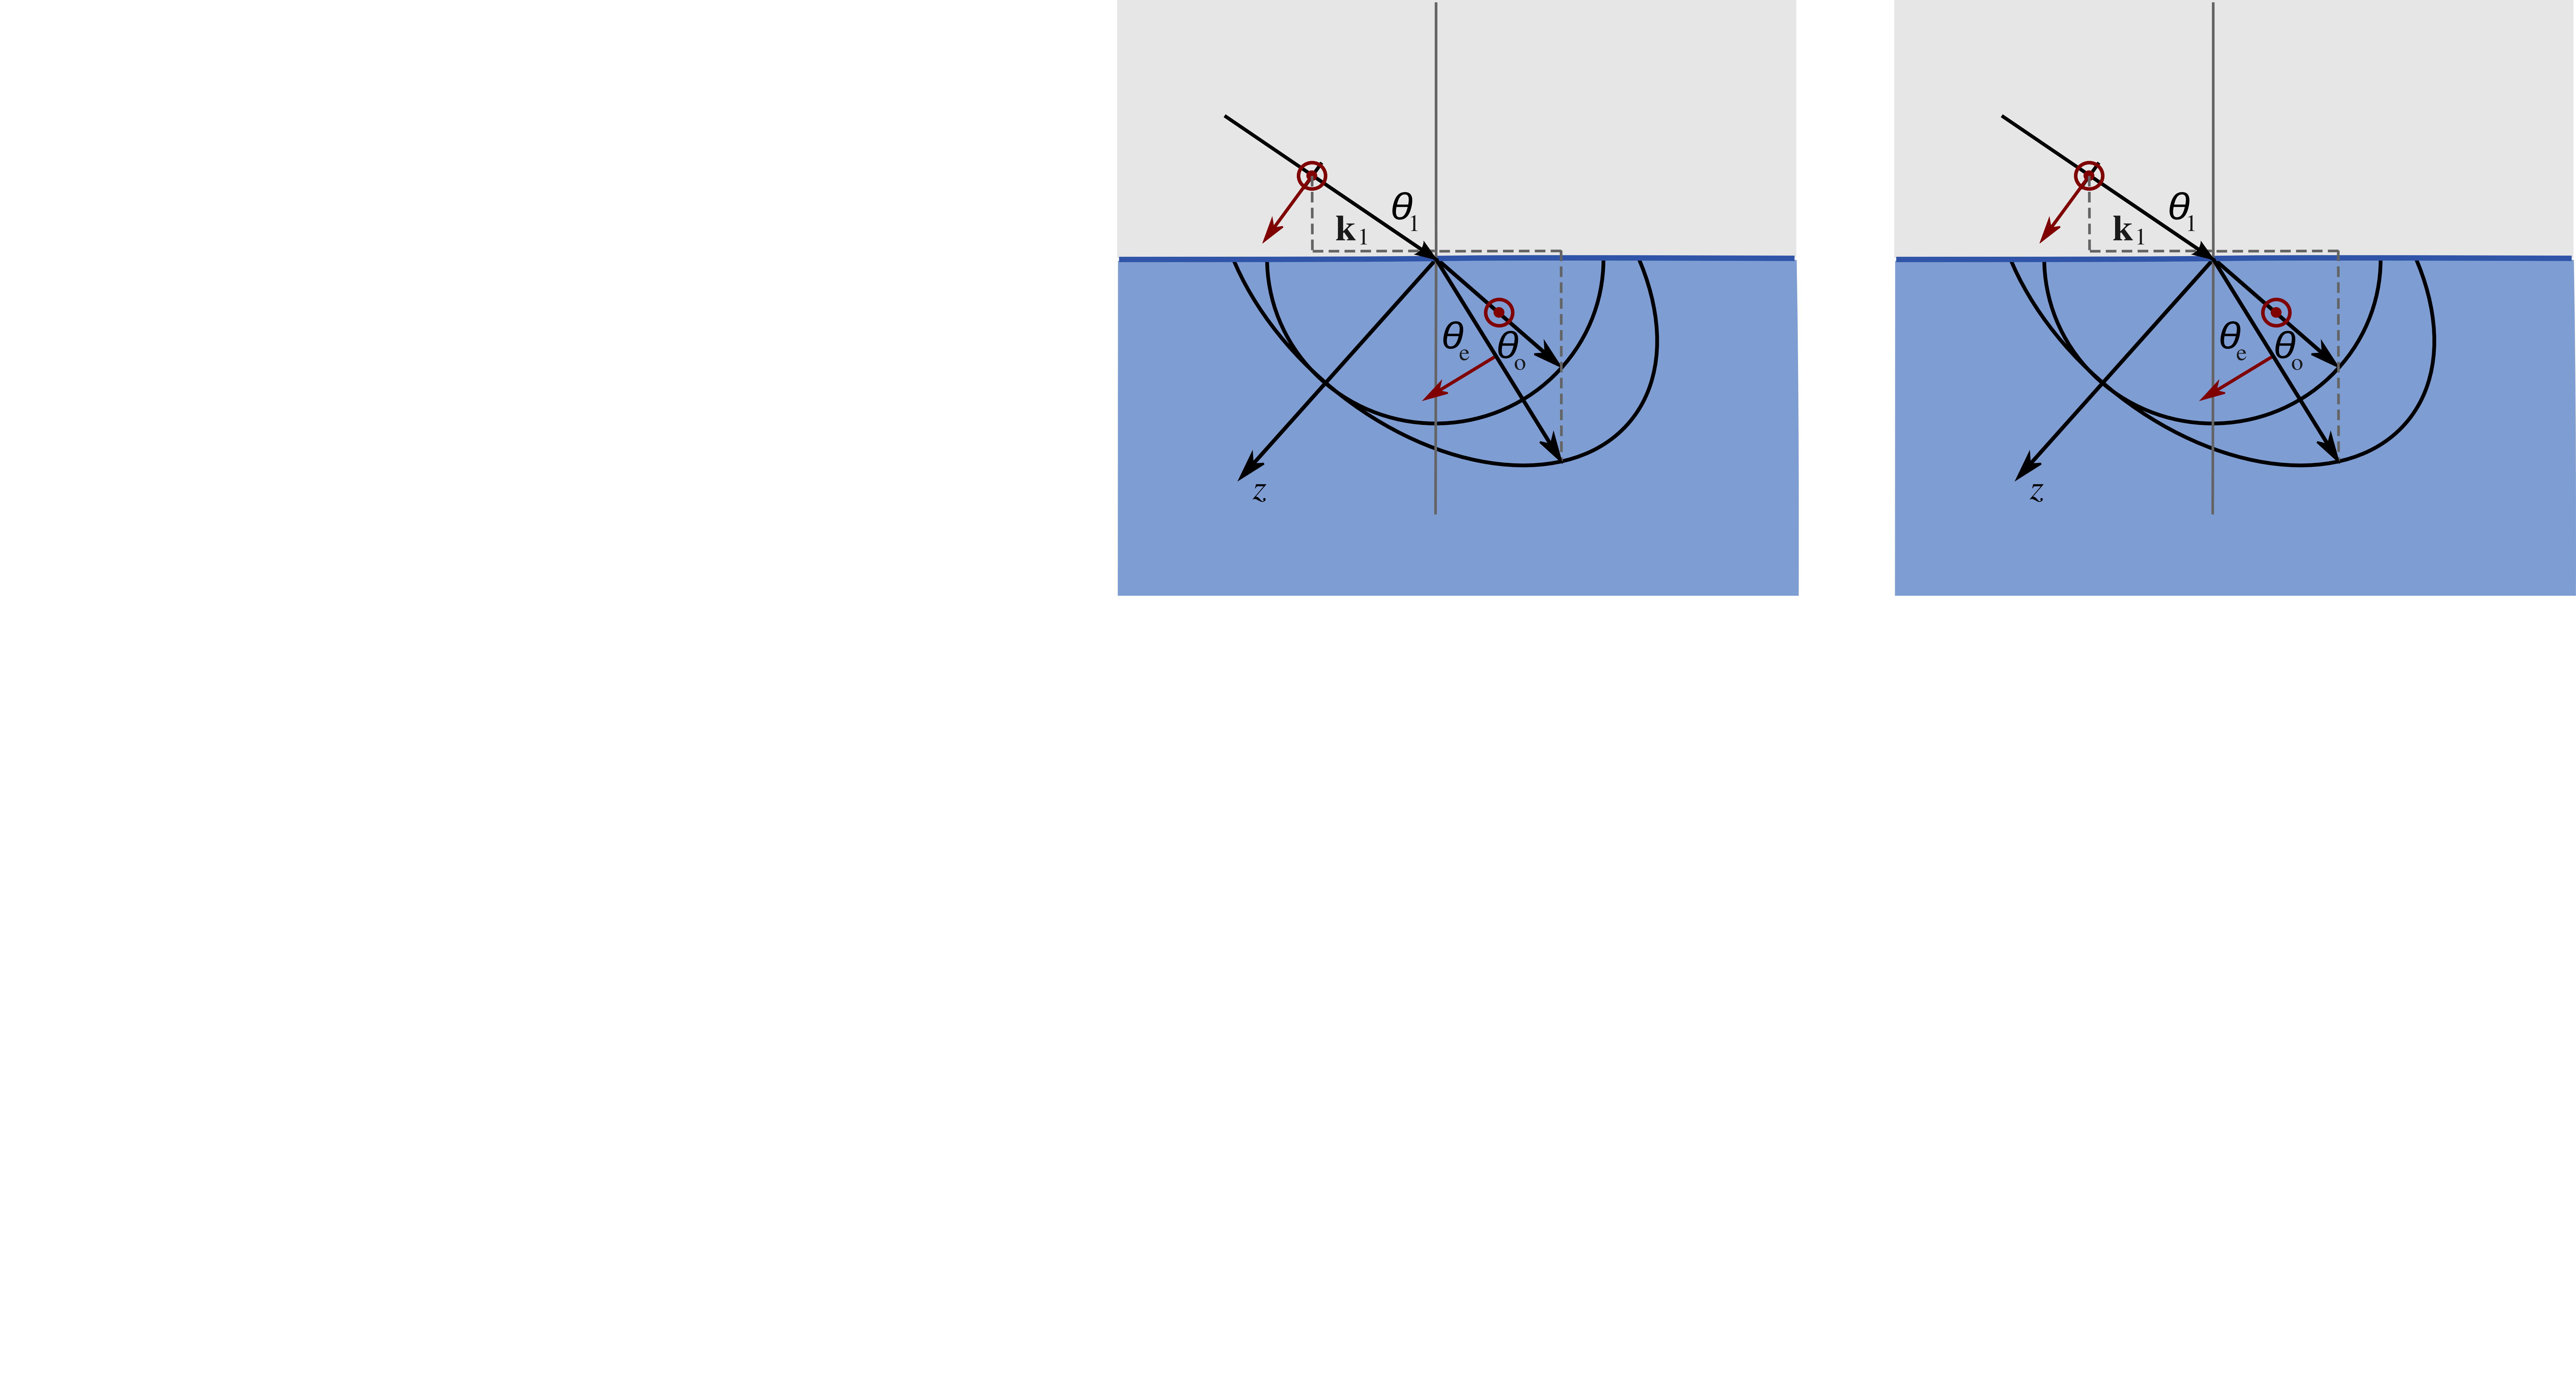
\includegraphics[width=12truecm]{dvojnilom.png}
\caption{\label{fig:dvolomnost}Dvolomnost omejenih snopov svetlobe (žarkov)
v dvolomnem kristalu pri pravokotnem vpadu.}
\end{figure}
 































\printindex

\end{document}
